\documentclass{article}
\usepackage[utf8]{inputenc}
\usepackage[spanish]{babel}



\usepackage{graphicx} %paquete básico para incluir gráficos
\usepackage{wrapfig} %paquete Wrapfig
\usepackage{float} % paquete para controlar entornos flotantes
\usepackage{pdfpages}% Paquete pdfpages incluye páginas completas de ficheros pdfs
\usepackage{lipsum} % Paquete para introducir texto 
\title{Taller yosigopublicando}

\author{yo}
\date{\today}

\begin{document}

\maketitle

\section{Introduction}

\begin{abstract}
Esto es la continuación del curso básico de \LaTeX{} con overleaf.
\end{abstract}
%%%%%%%%%%%%%%%%%%%%%%%%%%%%%%%%%%%%%%%%%%%%%%%%%%%%%%
\section{Inclusión de Gráficos}
\lipsum % Comando para inserta texto para rellenar.

{\bf Final lipsum 1}

\begin{figure}[h]
    \centering
    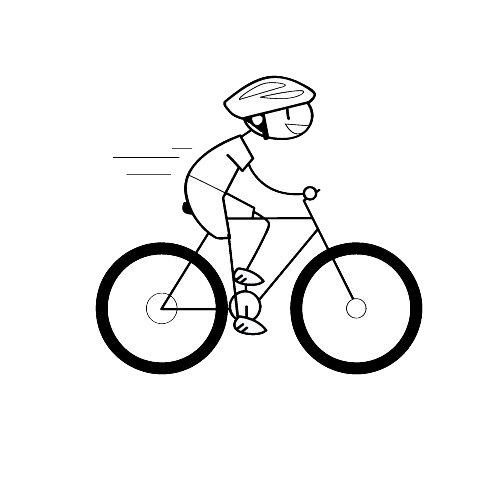
\includegraphics[height=5cm,angle=25]{graficos/ciclista.png}
    \caption{Una imagen simple en entorno Figure}
    \label{fig:1}
\end{figure}

\begin{wrapfigure}{r}{0.45\textwidth}
 \vspace{-0.5cm}
 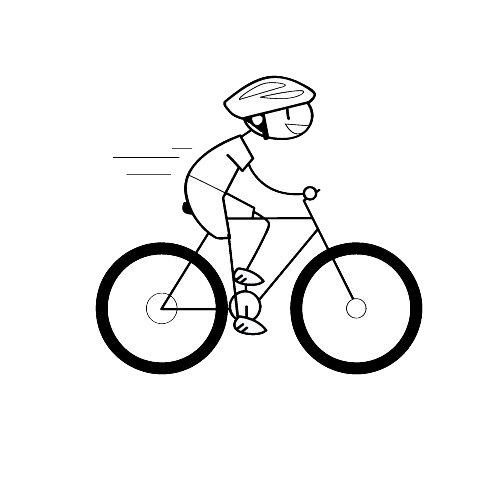
\includegraphics[trim= 0mm 15mm 0mm 8mm,clip,width=0.4\textwidth]{graficos/ciclista.png}
    \caption{Una imagen simple en entorno Wrapfigure}
\end{wrapfigure}

\lipsum

{\bf Final lipsum 2}

\begin{figure}
    \centering
    \frame{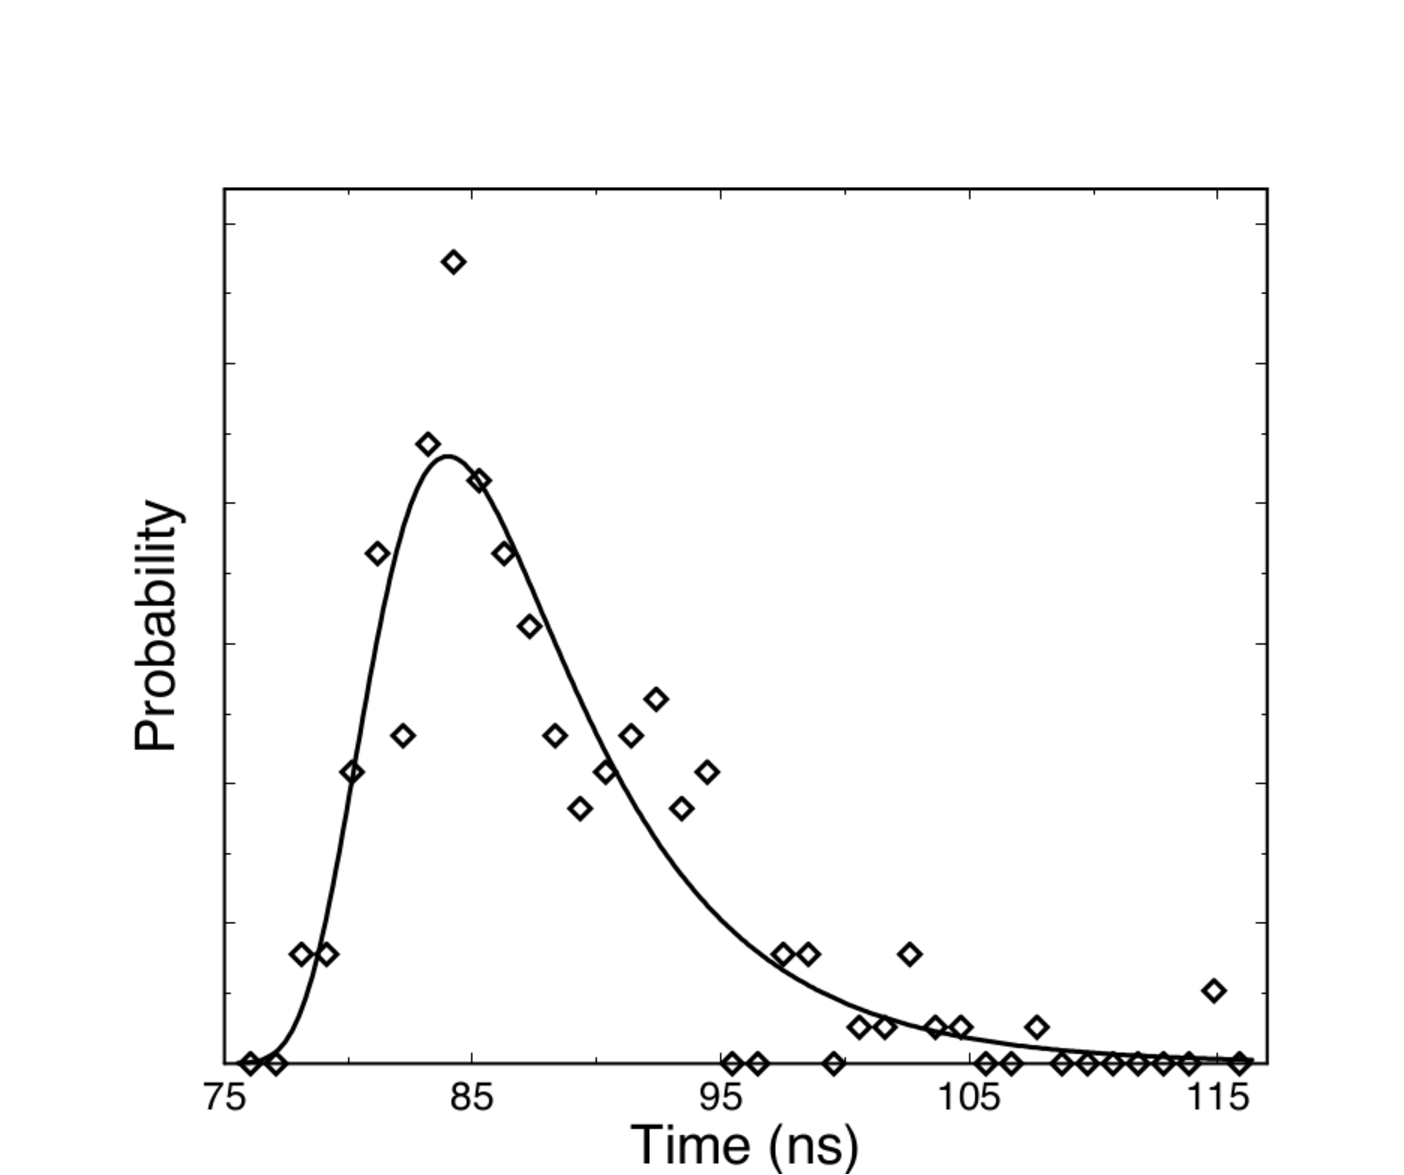
\includegraphics[width=0.45\textwidth]{graficos/fig_9Vis.pdf}}
    \frame{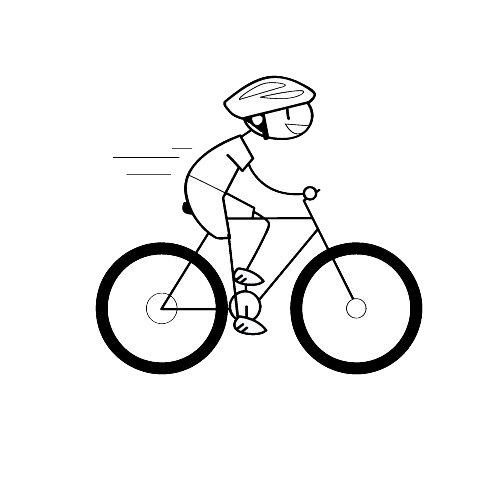
\includegraphics[width=0.45\textwidth]{graficos/ciclista.png}}
    \caption{Dos imágenes contiguas}
    \label{fig:2}
\end{figure}
\lipsum

{\bf Final lipsum 3}

%\begin{figure}
%    \centering
    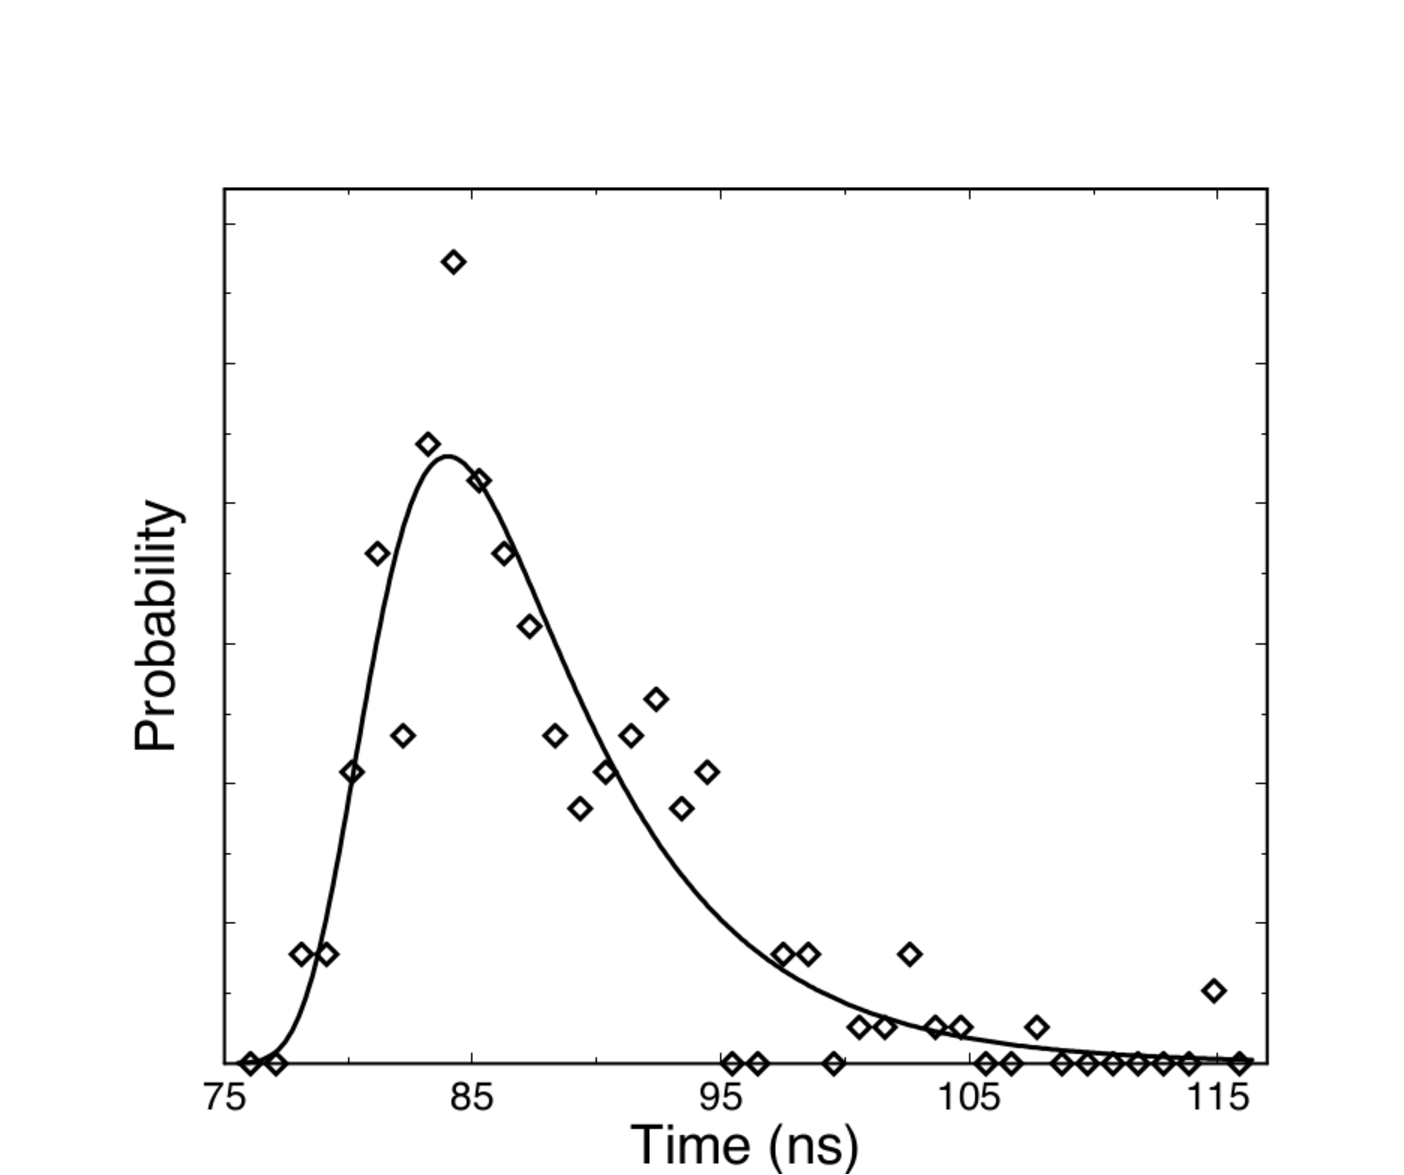
\includegraphics[trim= 0mm 0mm 0mm 30mm,clip,angle=0,width=0.45\textwidth]{graficos/fig_9Vis.pdf}
    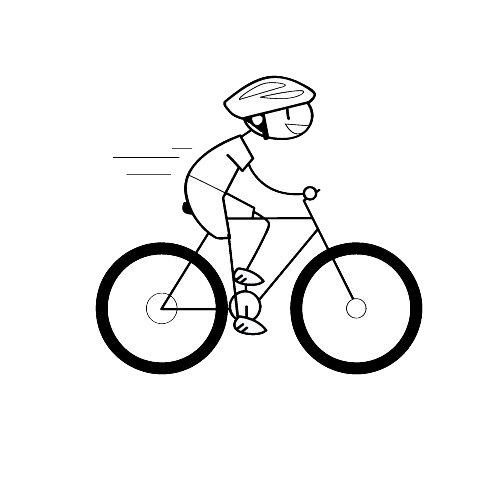
\includegraphics[trim= 0mm 15mm 0mm 5mm,clip,width=0.45\textwidth]{graficos/ciclista.png}
%    \caption{Dos imágenes contiguas recortadas para que queden a nivel.}
%    \label{fig:3}
%\end{figure}
\lipsum

{\bf Final lipsum 4}

\begin{figure}[H]
    \centering
    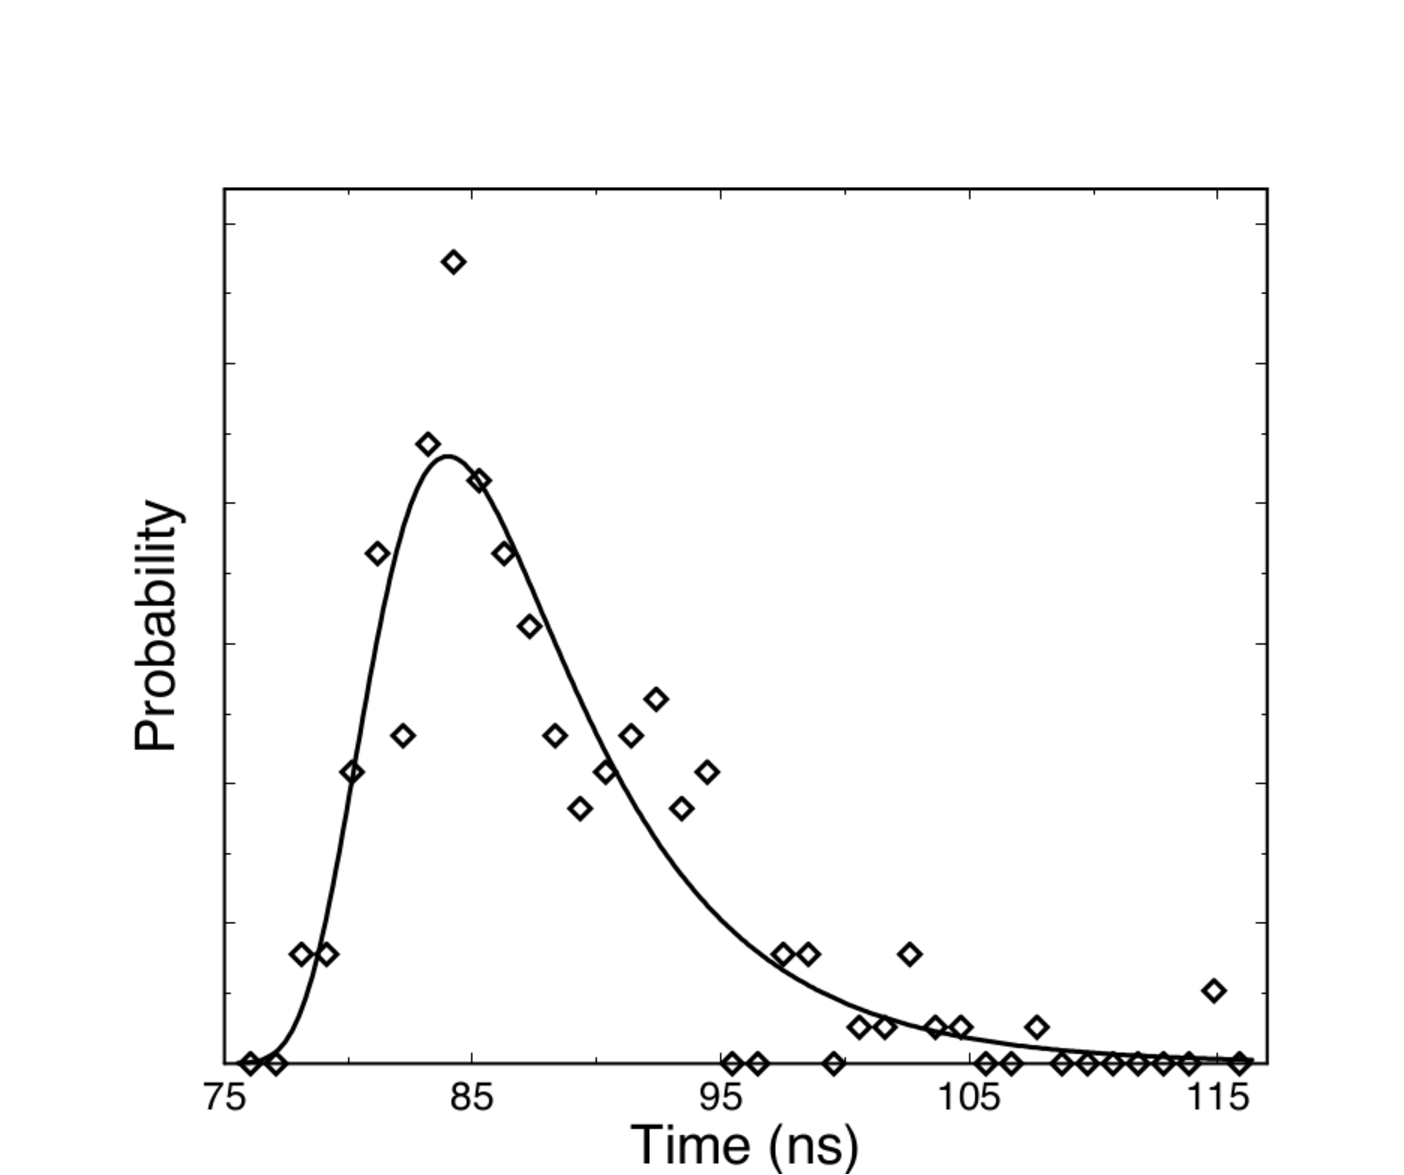
\includegraphics[trim= 0mm 0mm 0mm 30mm,clip,angle=0,width=0.7\textwidth]{graficos/fig_9Vis.pdf}
    \put(-80,150){v=20km/h}
    \put(-100,10){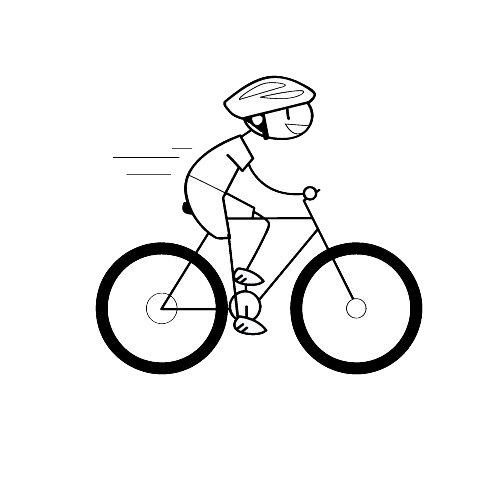
\includegraphics[angle=-7,scale=0.4]{graficos/ciclista.png}}
   % 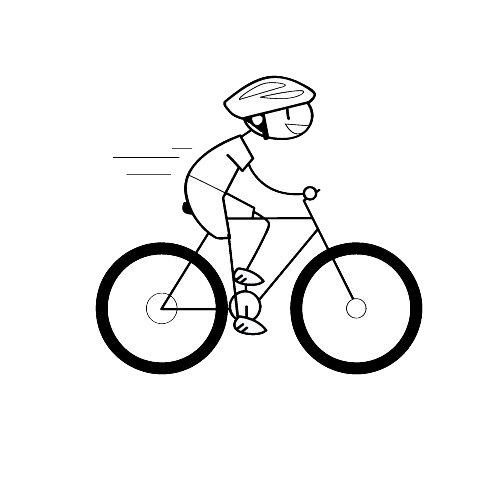
\includegraphics[trim= 0mm 15mm 0mm 5mm,clip,width=0.45\textwidth]{graficos/ciclista.png}
    \caption{Imágen y texto superpuesto.}
    \label{fig:4}
\end{figure}

\lipsum

{\bf Final lipsum 5}

\begin{figure}[H]
\centering
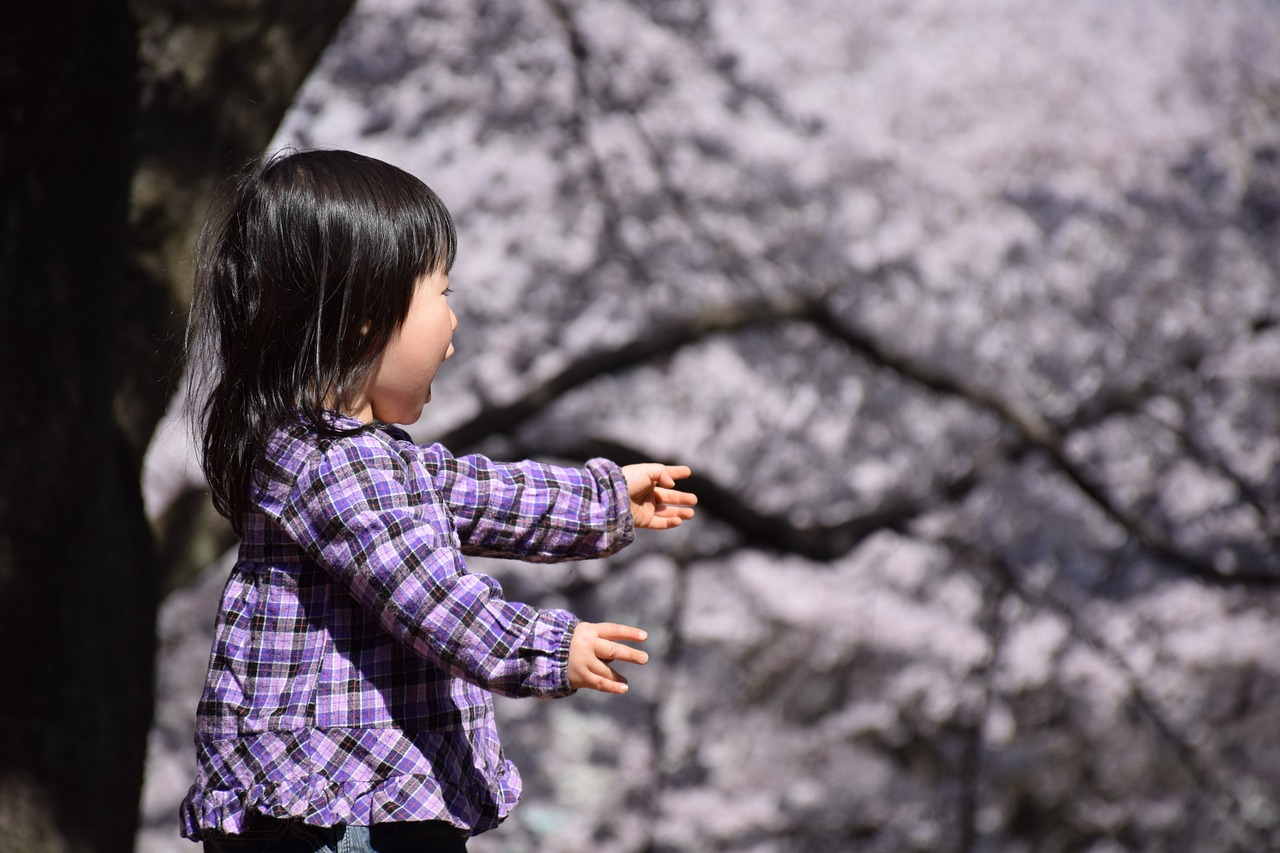
\includegraphics[trim = 50mm 0mm 190mm 40mm, clip,width=5cm]{./graficos/sorpresa}
\hspace{-0.35cm}
\reflectbox{
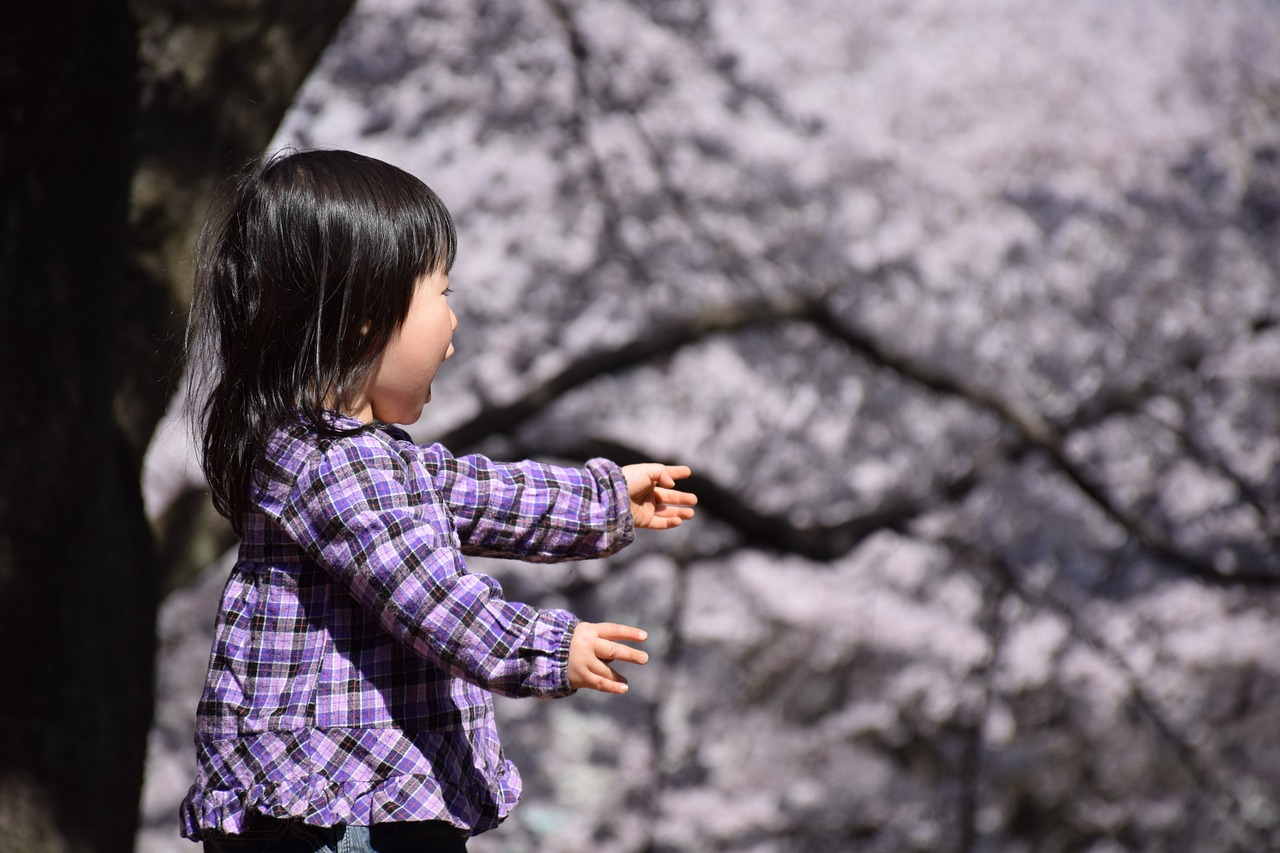
\includegraphics[trim = 50mm 0mm 190mm 40mm, clip,width=5cm]{./graficos/sorpresa}
}
\caption{Montaje con imagen recortada y reflejada.}
\label{fig:5}
\end{figure}

%%%%%%%%%%%%%%%%%%%%%%%%%%%%%%%%%%%%%%%%%%%%%%%%%%%%%%%%%%%%%
\section{Inclusión de páginas pdf}

\includepdf[]{graficos/Diploma.pdf}


\end{document}